\section{Practical Deployment}\label{sec-deployment}

As mentioned previously, we have running implementations of all
Seattle components on nodes on the public Internet, including
many instances we neither control nor operate. These latter
implementations have been
contributed to our Clearinghouse's resource pool by volunteers.
Apart from the numbers we report below, we do not have any
insight on offspring projects that reuse our open-source software
base, but set up their own independent deployments.
Seattle has no tracking code besides what an operating Clearinghouse
needs to support the sandboxes it controls.

To assess the current scale and size of Seattle, we report
statistics from the \gls{IP} addresses contacting our Software
Updater service. This service is contacted
by all installations that Seattle's main Installer Builder shipped
to end-user devices, and has reported downloads from over 40,000
different \gls{IP} addresses over our eight years of deployment history.
This metric is not perfect: it undercounts multiple devices behind
a \gls{NAT} gateway, and overcounts devices that change their
\gls{IP} address frequently (such as mobile nodes). However, it
gives an impression of the scale of our deployment.

Attempting to reverse-resolve these \gls{IP} addresses to \gls{DNS}
names yields no result for about 50\% of addresses; resolves to
names that belong to home Internet providers for another 30\%; and to university
machines for the remaining 15\%. The latter likely includes students, since they
often use on-campus computers in classrooms or labs. Note also that the number
of online nodes (and thus sandboxes) varies over time, as device owners
turn off or suspend their devices as they move, or as their daily
routines start and end.
Figure~\ref{fig:map} plots a world map of Seattle nodes, with the
colors encoding the approximate node density in an area.
Node locations were generated from GeoIP data.
It shows that Seattle has notable user bases outside of the
United States (where it was originally developed),
particularly in Central Europe and China.

Since its inception,
more than 4,000 experimenters have used Seattle's Clearinghouse
to request access to resources on remote devices. We attribute this
to the fact that our Clearinghouse offers ten free sandboxes for
every registered user, and contributing one's own resources counts
as a ``credit'' to use more remote sandboxes in turn.
Resource credits have proven a valuable incentivation strategy
to push the adoption of Seattle.

While offering generous resources to bootstrap experiments,
Seattle has also benefitted greatly from generous contributions
of code, documentation, tutorials, and libraries from more than 100
contributors at 32 institutions all over the world.
Seattle strives to make contributing easy. All of its components
are open-source software, and thus easy to inspect, adapt, and
reuse in other contexts.

Sensibility Testbed~\cite{zhuang2014sensibility} has been particularly
successful in adapting and reusing Seattle components. It extends
Seattle's sandbox type so as to allow access
to sensors on Android smartphones and tablets. Furthermore, its
Device Manager includes an additional \gls{GUI} in the form of
a native Android app. Sensibility Testbed's Clearinghouse implements
special policies not found in Seattle. An experimenter requesting
sandboxes on Sensibility Testbed must first complete
an \gls{IRB} approval process, which ensures that the experiment conducted
does not impact the privacy of device owners involved.


\begin{figure}
  \centering
  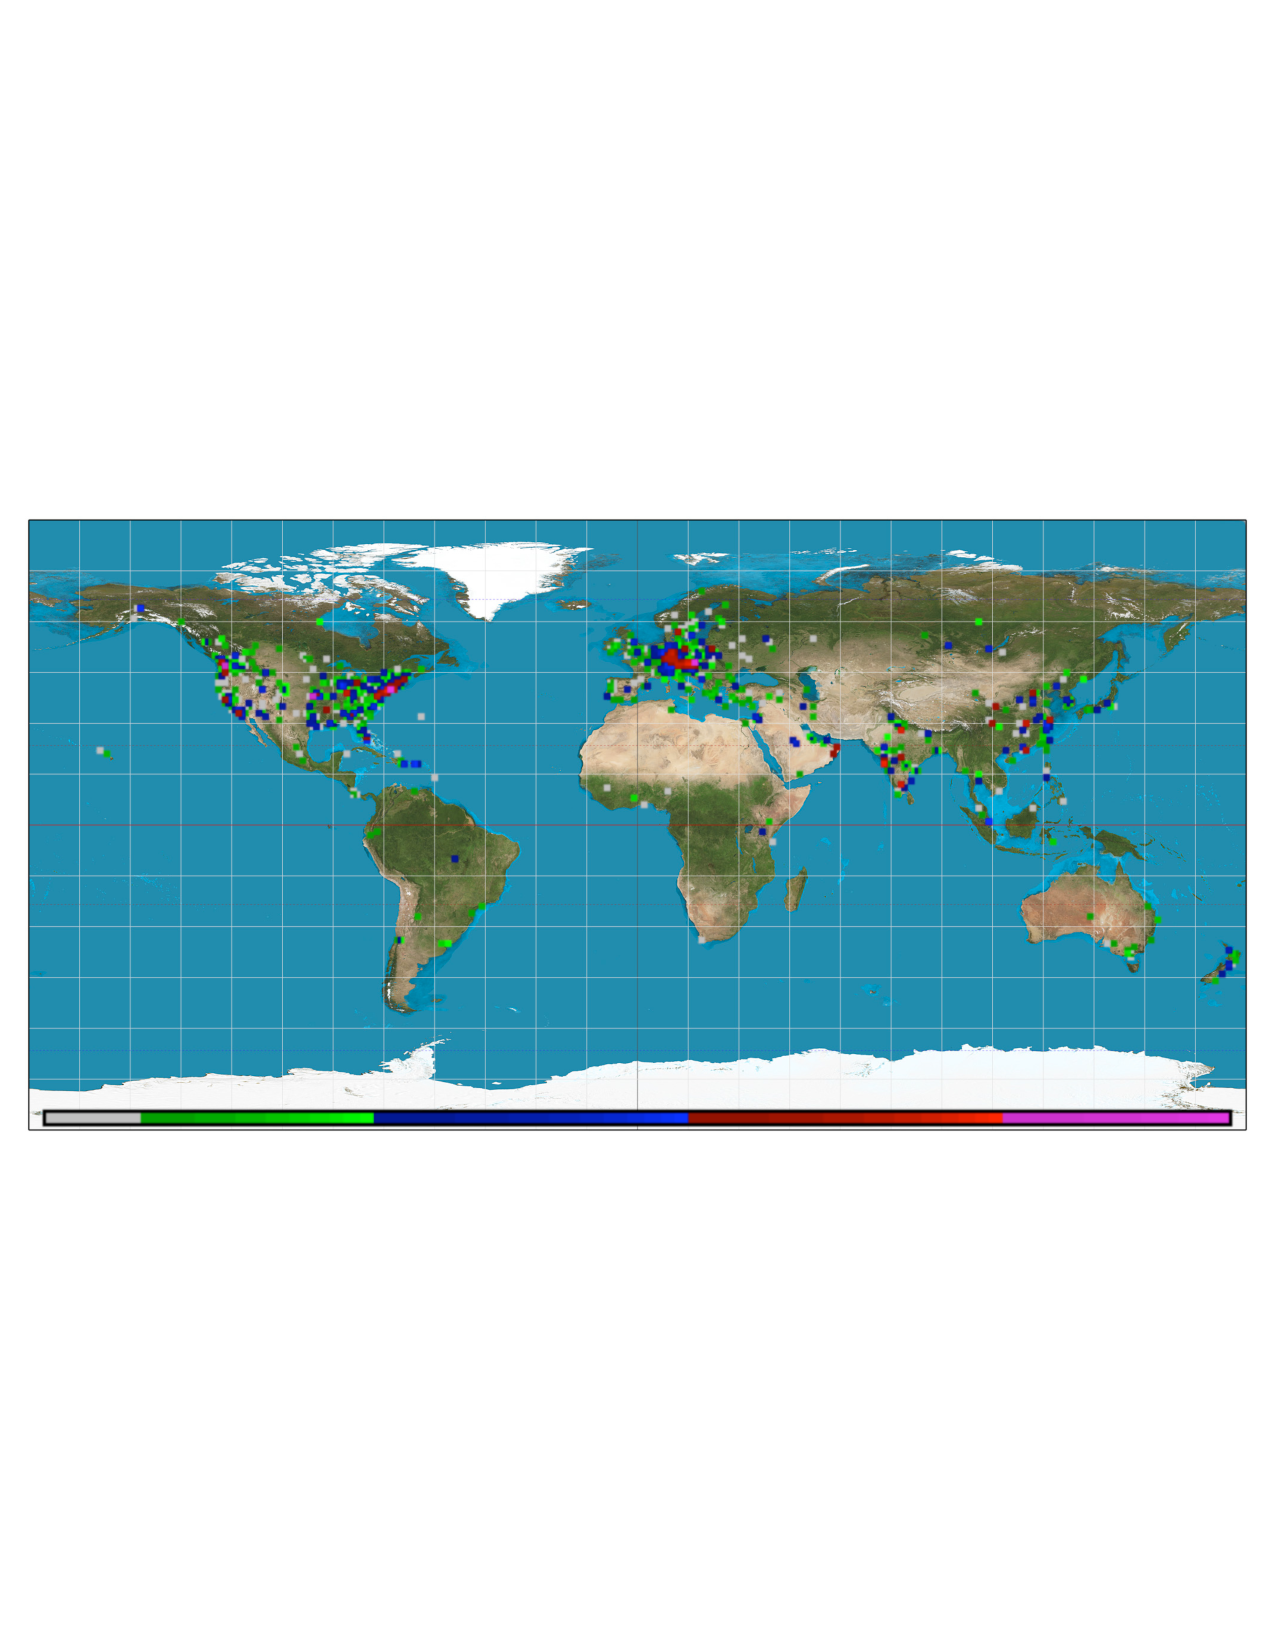
\includegraphics[width=\columnwidth]{figures/finishedmap_ipinfo_small.pdf}
  \caption{World map of Seattle node locations. Color shows approximate density from low (grey) to high (magenta).}
  \label{fig:map}
\end{figure}
